\section{Tìm kiếm lân cận rộng}

\begin{figure}[H] % places figure environment here   
  \centering % Centers Graphic
  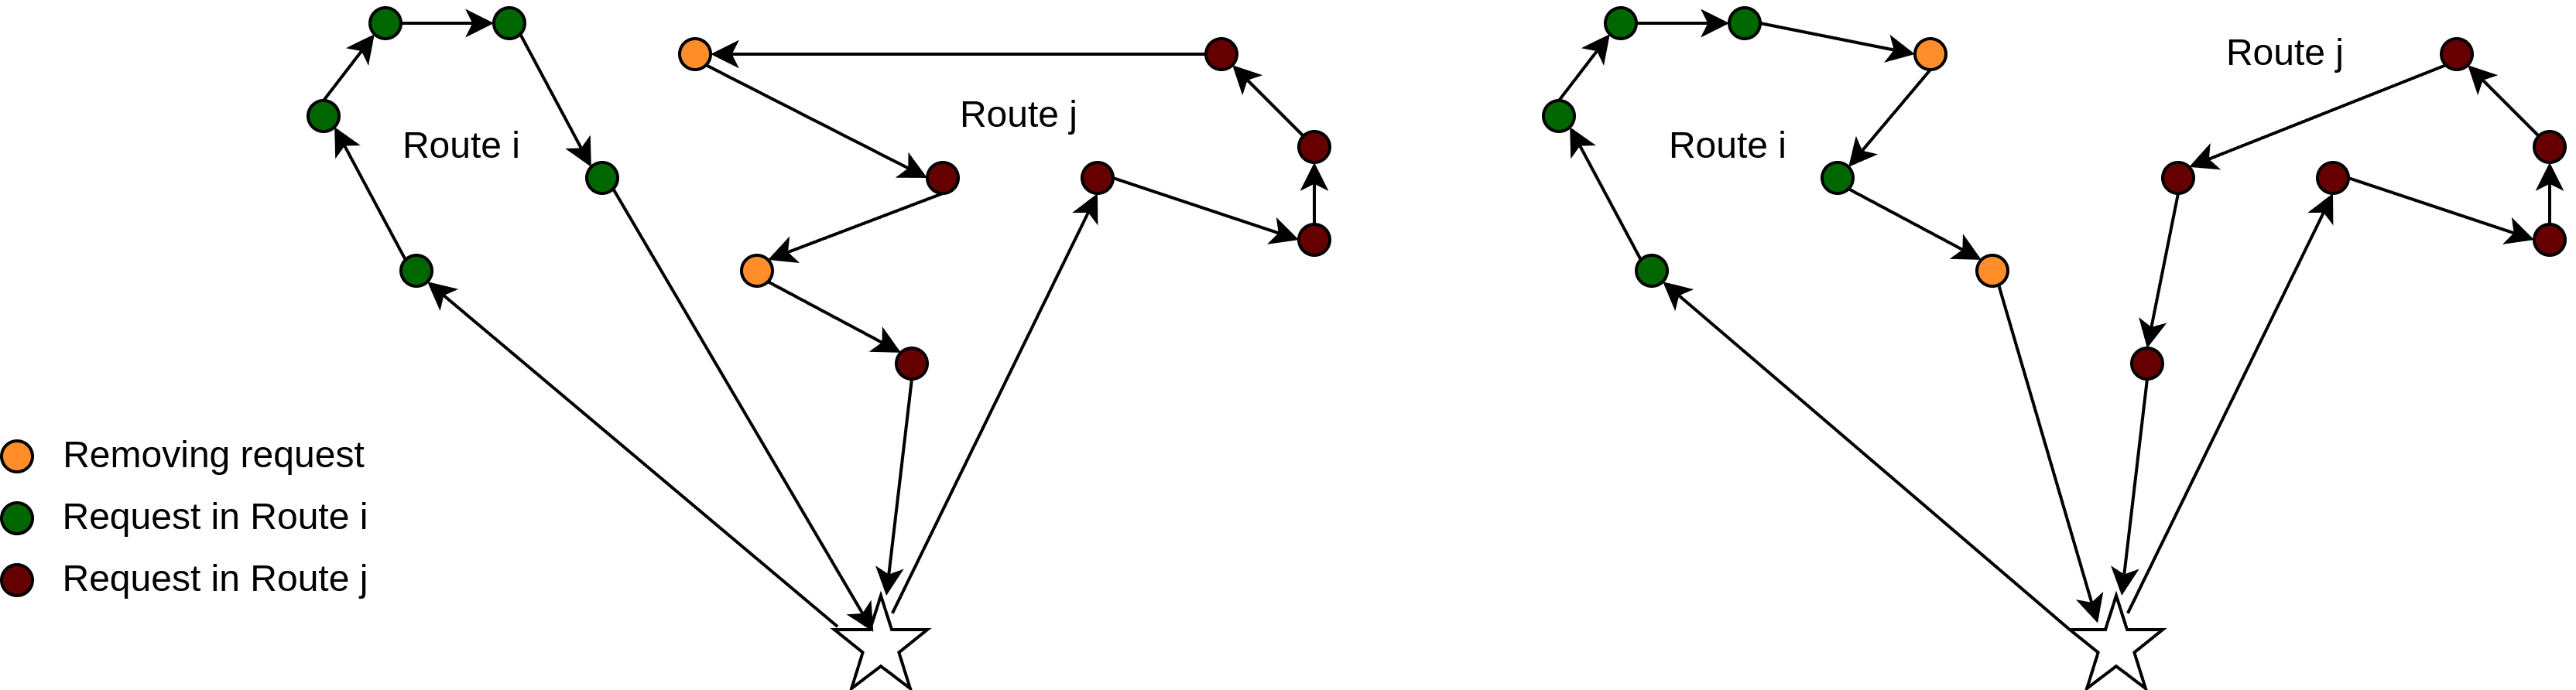
\includegraphics[width=0.9\textwidth]{figures/ALNS-paradim.png} 
  % \includesvg[scale=1]{figures/core-object}
  \caption{Lược đồ LNS} 
  \label{fig:lns_paradim}
\end{figure}

Phương pháp tìm kiếm lân cận rộng (Large neighbourhood search - LNS) được trình bày bởi Shaw (1998) \cite{shaw1998using} thuộc lớp các thuật toán tìm kiếm lân cận. LNS dựa trên việc liên tục bỏ đi yêu cầu và tối ưu lại nghiệm. Nghĩa là một số yêu cầu được bỏ đi khỏi tuyến (theo một tiêu chí nào đó) và được thêm lại vào các tuyến (khác) với mục đích làm giảm hàm mục tiêu hay khám phá ra nghiệm mới thỏa mãn các ràng buộc.

\begin{algorithm}
  \label{alg:lns}
	\caption{LNS Heuristic} 
	\begin{algorithmic}[1]
        \Require $s \in \text{\{nghiệm chấp nhận được\}}, q \in \mathbb{N}$
        \State nghiệm $s_{best} = s$;
				\Repeat
					\State $s'=s$;
					\State bỏ $q$ yêu cầu từ $s'$;
					\State thêm lại các yêu cầu đã bỏ đi vào $s'$;
					\If{$f(s') < f(s)$}
						\State $s_{best} = s'$;
					\EndIf
					\If{$accept(s',s)$}
						\State $s=s'$;
					\EndIf
				\Until{đạt điều kiện dừng}\\
				\Return $s_{best}$;
	\end{algorithmic} 
\end{algorithm}

Thuật toán giả định rằng nghiệm ban đầu \textit{s} đã được khởi tạo (thường bằng một heuristic đơn giản). Tham số \textit{q} xác định phạm vi tìm kiếm. 

Dòng 4 và 5 của thuật toán là phần thú vị của heuristic. Ở dòng 4, một số yêu cầu được loại bỏ khỏi phương án hiện tại \textit{s'}, các yêu cầu lại được thêm vào ở dòng 5. Hiệu năng cũng như sự mạnh mẽ của heuristic phụ thuộc vào sự lựa chọn chiến thuật bỏ và thêm lại các yêu cầu. Trong các bài trước đó về LNS cho VRPTW và PDPTW (Shaw (1997) \cite{shaw1997new}; Bent, Van Hentenryck (2003) \cite{bent2003two}) các phương pháp \textit{gần tối ưu} được sử dụng để thêm lại các yêu cầu. Mặc dù các cách thêm lại yêu cầu heuristic thường có chất lượng không tốt, nhưng chất lượng tổng thể của LNS heurustic lại rất tốt, bởi vì các bước "tệ" được tạo ra bởi heuristic thêm lại yêu cầu dẫn đến sự đa dạng hóa quá trình tìm kiếm. Nói cách khác LNS cho phép tìm kiếm đa dạng nghiệm trong vùng lân cận để tránh bị bẫy trong một nghiệm tối ưu địa phương.

Trong phần còn lại, LNS cập nhật phương án tốt nhất (hiện tại) và tìm kiếm phương án mới (tốt hơn). Tiêu chí chấp nhận đơn giản nhất là chỉ chấp nhận các nghiệm tốt hơn (có chi phí nhỏ hơn) nghiệm hiện tại. Tiêu chí này đã được sử dụng trong triển khai LNS của Shaw (1997) \cite{shaw1997new}. Dòng 10 kiểm tra điều kiện dừng đã đạt được hay chưa.

Tham số $q \in \{0,...,n\}$ xác định kích cỡ tập lân cận. Ta cần $q > 0$ vì khi không có yêu cầu nào được bỏ đi thì thuật toán không hoạt động. Mặt khác nếu $q = n$, thì bài toán được giải luôn qua mỗi vòng lặp. Nói chung, $q$ càng lớn thì càng dễ di chuyển quanh không gian nghiệm, tuy nhiên khi $q$ lớn dần lên thì bước thêm lại yêu cầu sẽ chậm hơn. Trong thực nghiệm, ta không sử dụng một con số $q$ cố định, chiến thuật chọn số $q$ được trình bày trong phần \ref{sec:num_rm_req}.

Ngoài ra, thay vì xem xét quá trình LNS như là một chuỗi hành động xoá và thêm lại, chúng ta có thể coi quá trình này là chuỗi hành động sửa lỗi. Cách nhìn này giúp chúng ta áp dụng chiến thuật này không chỉ cho bài toán VRP mà còn có thể áp dụng cho các bài toán tối ưu tổ hợp khác nữa. Chính vì tính chất linh hoạt này, tác giả đã lựa chọn LNS làm nền tảng cho phương pháp tìm kiếm lân cận trong luận văn này.

\subsection{Thuật toán hủy}

\subsubsection*{Phương pháp xóa tệ nhất}
Cho 1 yêu cầu $i$ được phục vụ bởi vài xe trong tập nghiệm $s$, chi phí của yêu cầu \textit{cost} được định nghĩa là hàm $cost(i,s)=f(s)-f_{-i}(s)$ với $f_{-i}(s)$ là chi phí của nghiệm mà không có yêu cầu $i$ (yêu cầu được xóa mà không chuyển đến hàng chờ). Chiến thuật ở đây là ta xóa đi những yêu cầu có chi phí cao và cố gắng thêm lại vào các tuyến với chi phí ít hơn.

Tuy nhiên chúng ta không xóa đi chính xác các yêu cầu có chi phí cao nhất mà thay vào đó chúng ta chọn ngẫu nhiên 1 yêu cầu có chi phí cao. Điều này được thực hiện để tránh việc xóa các yêu cầu có chi phí cao nhất liên tục và thuật toán bị bẫy trong một nghiệm tối ưu cục bộ.

\begin{algorithm}
	\label{alg:worst_removal}
	\caption{Worst Removal}
	\begin{algorithmic}[1]
		\Require $s \in {solutions}, q \in \mathbb{N}, p \in \mathbb{R}_{+}$
		\While {$q > 0$}
		\State Array: \textit{L} = All planned requests \textit{i}, sorted by descending \textit{cost(i,s)};
		\State choose a random number \textit{y} in the interval $[0, 1)$;
		\State request: $r = L\left[ y^p |L| \right]$;
		\State remove r from solution s;
		\State $q = q-1$;
		\EndWhile
	\end{algorithmic}
\end{algorithm}

\subsubsection*{Phương pháp xóa ngẫu nhiên}
Thuật toán xóa ngẫu nhiên đơn giản chọn ngẫu nhiên $q$ yêu cầu và loại bỏ chúng khỏi nghiệm hiện tại. Kỹ thuật này có thể coi là 1 trường hợp đặc biệt của phương pháp xóa Shaw với $p=1$.

\subsubsection*{Phương pháp xóa Shaw}
Phương pháp xóa này được phát triển bởi Shaw (1997, 1998) \cite{}. Cách trình bày trong phần này đã được chỉnh sửa lại để phù hợp với VRPTW. Ý tưởng chung là xóa bỏ các yêu cầu có "liên quan", vì chúng ta hy vọng sẽ dễ dàng thêm lại các yêu cầu tương tự với nhau để tạo ra các nghiệm mới có thể tốt hơn. Nếu chúng ta chọn xóa bỏ các yêu cầu rất khác nhau, thì sau đó, việc thêm các yêu cầu mới sẽ không nhận lại được điều gì do các yêu cầu này có thể chỉ được thêm vào tại vị trí ban đầu của chúng hoặc ở các vị trí tệ. Mức độ liên quan giữa 2 yêu cầu \textit{i} và \textit{j} được định nghĩa dựa trên chỉ số độ liên quan $R(i,j)$. Chỉ số này càng thấp thì 2 yêu cầu càng "giống" nhau.

Chỉ số độ tương đồng được sử dụng bao gồm phụ thuộc vào ba điều kiện là khoảng cách, thời gian, khối lượng. Các điều kiện này được đánh trọng số và ký hiệu lần lượt là $\varphi$, $\chi$ và $\psi$. Chỉ số độ tương đồng được tính như sau
\begin{equation}
	\label{eq:shaw_related}
	R(i,j) = \varphi d_{ij} + \chi |t_{i}-t_{j}| + \psi|l_i - l_j|
\end{equation}
$d_{ij}$ là khoảng cách từ $i$ tới $j$, $t_i$ là thời gian khi đến địa điểm $i$, $l_i$ là tải của xe tại $i$.

Mức độ liên quan được sử dụng để xóa các yêu cầu được mô tả trong Algorithm 3. Ban đầu, một yêu cầu được chọn ngẫu nhiên. Trong các vòng lặp tiếp theo, thuật toán sẽ thực hiện xóa các yêu cầu "giống" với các yêu cầu đã được xóa. Tham số $p \geqslant 1$ biểu diễn cho sự ngẫu nhiên trong cách lựa chọn yêu cầu (\textit{p} càng thấp thì độ ngẫu nhiên càng cao).

\begin{algorithm}
	\caption{Shaw Removal}
	\begin{algorithmic}[1]
		\Require $s \in {solutions}, q \in \mathbb{N}, p \in \mathbb{R}_{+}$
		\State request: r = a randomly selected request from s;
		\State set of requests: $\mathbb{D}=\{r\}$;
		\While {$|\mathbb{D}| < q$}
		\State r = a randomly selected request from $\mathbb{D}$;
		\State Array: L = an array containing all request from s not in $\mathbb{D}$;
		\State sort \textit{L} such that $i<j \Rightarrow R(r, L\left[ i \right]) < R(r, L\left[ j \right])$;
		\State choose a random number \textit{y} from the interval [0, 1);
		\State $\mathbb{D}=\mathbb{D}\cup {L \left[ y^p|L| \right]}$
		\EndWhile
		\State remove the requests in $\mathbb{D}$ from \textit{s};
	\end{algorithmic}
\end{algorithm}

Tinh thần của thuật toán Shaw là cố gắng bỏ đi top các yêu cầu có độ đo liên quan $R(i,j)$ nhỏ. Top các yêu cầu này được kiểm soát bằng tham số $p$. Tuy nhiên việc sắp xếp các yêu cầu (mảng $L$) theo thứ tự tăng dần của $R(r, L[i])$ là phép toán tốn chi phí. Trong thực tế cài đặt chúng ta có thể sử dụng cấu trúc dữ liệu \textit{min heap} để lấy ra top các yêu cầu có độ đo liên quan nhỏ nhất.

\subsubsection*{Hủy tuyến}
Thuật toán hủy tuyến được tác giả đề xuất trong luận văn này. Tinh thần chung của thuật toán là chúng ta cố gắng bỏ đi toàn bộ yêu cầu trên một hoặc một vài tuyến đường nào đó. Việc bỏ đi cả tuyến cũng tương đương với việc làm giảm số xe cần để phục vụ khách hàng. Mục tiêu của CVRPTW là giảm tổng khoảng cách di chuyển và nghiệm thu được phải thỏa mãn các ràng buộc về tải trọng, số xe cũng như khung thời gian. Tuy nhiên, trong thực tế vận hành của một doanh nghiệp, giảm bớt được số xe phục vụ là điều rất có ý nghĩa bởi chi phí mua (thuê) xe là đắt đỏ so với việc di chuyển xa hơn một vài phần trăm.

Áp dụng tư tưởng \textit{greedy}, tác giả cho rằng các tuyến nên được bỏ đi là các tuyến có chi phí trung bình trên mỗi khách hàng cao. Chúng ta kì vọng có thể thêm lại các khách hàng đó vào các tuyến khác "thoáng" hơn hay là chi phí trung bình trên mỗi khách hàng thấp hơn.
\begin{equation}
	\label{eq:destroy_route}
	\text{avg\_cost}(r, s) = \frac{\text{cost}(r, s)}{\text{size}(r)-1}
\end{equation}
với $r$ là tuyến được chọn, $\text{cost}(r,s)$ là chi phí của tuyến $r$ trong nghiệm $s$, $\text{size}(r)$ là số phần tử của tuyến $r$. Lưu ý rằng tuyến bắt đầu và kết thúc tại nút $0$.

Ngoài ra để tránh việc bỏ đi tuyến "tệ" một cách cứng nhắc, tác giả đưa vào một nhiễu nhỏ.\begin{equation}
	\label{eq:destroy_route}
	\text{avg\_cost}(r, s) = \frac{\text{cost}(r, s)}{\text{size}(r)-1} + \lambda p d_{max}
\end{equation}
với $d_{max}$ là khoảng cách lớn nhất giữa hai yêu cầu, $p$ là một số ngẫu nhiên trong khoảng $(-1,1)$ và $\lambda$ là một hằng số điều khiển.

Ngoài ra, chúng ta cũng không muốn bỏ đi các tuyến đang phục vụ nhiều yêu cầu vì khi thêm lại thuật toán sẽ mất rất nhiều thời gian. Chính vì thế, tác giả chỉ bỏ đi những tuyến có số yêu cầu ít hơn số yêu cầu trung bình trên mỗi tuyến của nghiệm hiện tại.

Cuối cùng, ta bỏ đi toàn bộ yêu cầu trên tuyến có số yêu cầu ít hơn số yêu cầu trung bình trên tất cả các tuyến và có chi phí trung bình trên mỗi yêu cầu cao nhất.
\subsection{Thuật toán sửa}

\subsubsection{Phương pháp tham lam cơ bản}
\label{sec:basic_greedy}
Heuristic tham lam cơ bản (\textit{basic greedy}) là một kỹ thuật xây dựng đơn giản (S. Ropke, D. Pisinger \cite{ropke2006adaptive}). Nó thực hiện tối đa $n$ lần lặp, chèn thêm một yêu cầu trong mỗi bước. Với $\Delta f_{i, k}$ biểu diễn cho sự thay đổi hàm mục tiêu bằng cách chèn thêm yêu cầu $i$ vào tuyến đường $k$ tại vị trí mà giá trị tăng thêm của hàm mục tiêu là nhỏ nhất. Nếu không chèn yêu cầu $i$ vào tuyến đường $k$ thì ta đặt $\Delta f_{i, k} = \infty$ và $c_i = \min_{k \in K}\{\Delta f_{i, k}\}$. Nói cách khác, $c_i$ là chi phí khi chèn thêm yêu cầu $i$ vào vị trí tốt nhất của nghiệm hiện tại, gọi là vị trí chi phí nhỏ nhất. Cuối cùng, ta chọn yêu cầu $i$ với $\min_{i \in U} c_i$ và chèn nó vào vị trí chi phí nhỏ nhất. Quá trình này tiếp tục cho đến khi tất cả các yêu cầu được thêm hoặc không còn yêu cầu nào nữa.

Trong mỗi vòng lặp, thuật toán chỉ thay đổi một tuyến đường (tuyến mà yêu cầu mới được thêm vào) và ta không cần phải tính toán lại chi phí chèn thêm trong tất cả các tuyến đường khác. Điểm này giúp tăng hiệu năng cho thuật toán. Đặc biệt nếu hàm mục tiêu là tổng quãng đường đi chuyển thì chúng ta có thể tính toán rất nhanh chi phí tăng thêm này. Giả sửa ta cần chèn thêm yêu cầu $u$ và giữa hai yêu cầu $i$ và $j$ trong tuyến đường $k$. Khi đó, chi phí tăng thêm của việc chèn thêm yêu cầu $u$ vào giữa $i$ và $j$ là $\Delta f_{u, i, j, k} = d_{iu} + d_{uj} - d_{ij}$.

Dễ dàng nhận thấy vấn đề với cách tiếp cận này là nó thường trì hoãn việc đặt các yêu cầu có chi phí cao cho các lần lặp cuối cùng, nơi chúng ta không có nhiều cơ hội cho việc chèn thêm yêu cầu vì nhiều tuyến đường đều đã kín. 

\subsubsection{Phương pháp tham lam với nhiễu ngẫu nhiên}

Để giải quyết một phần hạn chế của phương pháp tham lam cơ bản, ta có thể thêm một chút nhiễu vào hàm mục tiêu (E. Demir, T. Bekta¸s và G. Laporte \cite{Demir2012}). Điều này giúp thuật toán có thể không chọn chèn yêu cầu vào tuyến làm tăng chi phí ít nhất mà có thể là ít thứ hai hoặc thứ ba (chẳng hạn). Nhiễu được cho bởi công thức
\begin{equation}
  \eta = \lambda p d_{\text{max}},
\end{equation}
với $\eta$ là nhiễu, $d_{\text{max}}$ là khoảng cách lớn nhất giữa hai yêu cầu, $p$ là một số ngẫu nhiên trong khoảng $(-1,1)$ và $\lambda$ là một hằng số điều khiển \footnote[1]{$\lambda$ được đặt mặc định bằng $1$ trong thực nghiệm.}. Sau đó ta gán
\begin{equation}
  \Delta f_{u, i, j, k} := \Delta f_{u, i, j, k} + \eta.
\end{equation}

\subsubsection{Phương pháp heuristic hối tiếc}
Heuristic hối tiếc (\textit{regret heuristic}) đã được sử dụng bởi J.-Y. Potvin và J.-M. Rousseau \cite{potvin1993parallel} cho VRPTW. Phương pháp này cố gắng cải thiện nhược điểm của kỹ thuật tham lam bằng cách kiểm tra lại kết quả sau khi chọn chèn thêm yêu cầu. Đặt $x_{ik} \in \{1, ..., m\}$ là biến biểu diễn tuyến đường cho yêu cầu $i$ có chi phí chèn thêm vào thấp thứ $k$, điều này có nghĩa là $\Delta f_{i, x_{ik}} \leqslant \Delta f_{i, x_{ik'}}$ với mọi $k \leq k'$. Sử dụng ký hiệu này, ta có thể biểu diễn $c_i$ từ phần \ref{sec:basic_greedy}, $c_i = \Delta f_{i, x_{i1}}$. Trong phương pháp này, chúng ta có thể định nghĩa một giá trị \textit{regret} $c_i^* = \Delta f_{i, x_{i2}} - \Delta f_{i, x_{i1}}$ . Nói cách khác, giá trị \textit{regret} là khoảng cách giữa chi phí của việc chèn thêm yêu cầu vào tuyến đường tốt nhất so với tuyến đường tốt thứ hai. Trong mỗi vòng lặp, thuật toán chọn ra yêu cầu $i$ thỏa mãn điều kiện $\max_{i \in V \setminus \{0\}} \{c_i^*\}$. Nói một cách không chính thống, chúng ta chọn việc chèn yêu cầu mà chúng ta sẽ "hối tiếc" nhất nếu không thực hiện nó ngay tại vòng lặp hiện tại.

Ta có thể mở rộng phương pháp này để định nghĩa một lớp các phương pháp heuristic hối tiếc gọi là phương pháp regret-k heuristic là một phương pháp mà mỗi lần thêm yêu cầu vào phương án cần phải thỏa mãn điều kiện
\begin{equation}
    \max\limits_{i \in V \setminus \{0\} } \{ \sum_{j=1}^k (\Delta f_{i, x_{ij}} - \Delta f_{i, x_{i1}}) \}.
\end{equation}
Nếu một vài yêu cầu không thể được chèn thêm vào ít nhất $m-k+1$ tuyến đường thì yêu cầu đó sẽ được chèn vào tuyến ít yêu cầu nhất. Nếu ta vẫn không thể chèn yêu cầu vào tuyến này thì ta sẽ chèn vào tuyến giúp tăng chi phí ít nhất. Yêu cầu được chèn vào vị trí (trong tuyến) làm tăng ít chi phí nhất. Với $k>2$ thì thuật toán sẽ tính toán chi phí của việc thêm vào một yêu cầu với $k$ tuyến đường tốt nhất và chèn yêu cầu mà khoảng cách chi phí giữa việc thêm nó vào tuyến đường tốt nhất với các tuyến đường tốt thứ $k-1$ là lớn nhất. 

Với việc xét tốp $k$ vị trí tốt nhất của mỗi yêu cầu, hiệu năng của \textit{regret-k} sẽ không tốt bằng \textit{basic greedy}. Để dễ hình dung, với $n$ vị trí có thể chèn yêu cầu, trong mỗi bước lặp của thuật toán, với \textit{basic greedy} ta cần duyệt $O(n)$ lần qua các vị trí để tìm ra vị trí chèn tốt nhất; với \textit{regret-k} nếu sử dụng heap ta mất $O(k \times n)$ lần duyệt để  lấy ra tốp $k$ và $O(k)$ lần duyệt nữa để lấy ra yêu cầu mà khoảng cách $\Delta f$ trong top-k lớn nhất. Trong thực tế cài đặt, tác giả sử dụng đến $k=5$ và regret-k chứng tỏ được nó là một phương pháp mạnh và đáng để đánh đổi một chút về mặt hiệu năng khi so sáng với regret-2 heristic hay thuật toán tham lam cơ bản.
\subsection{Tiêu chí chấp nhận nghiệm}

Các tiêu chí chấp nhận nghiệm được tóm lược qua bảng \ref{tab:acceptance}

\begin{table}[caption={Tiêu chí chấp nhận nghiệm.}, label=tab:acceptance]
  \begin{tabularx}{\textwidth}{|l|X|}
    \hline
    Phương pháp & Mô tả \\ \hline
    \makecell[l]{Bước ngâu nhiên \\ (Random Walk)} & Mọi nghiệm $s'$ đều được chấp nhận \\ \hline
    \makecell[l]{Chấp nhận tham lam \\ (Greedy Acceptance)} & Nghiệm $s'$ được chấp nhận nếu chi phí của nó là nhỏ hơn so với nghiệm hiện tại \\ \hline
    \makecell[l]{Mô phỏng luyện kim \\ (Simulated Annealing)} & Mọi nghiệm cải thiện $s'$ được chấp nhận. Nếu $c(s') > c(s)$ thì $s'$ được chấp nhận với xác suất $\exp \{ \frac{c(s) - c(s')}{T} \}$ với $T$ là nhiệt độ. Nhiệt độ $T$ giảm sau mỗi vòng lặp với một hệ số $\Phi$ \\ \hline
    \makecell[l]{Chấp nhận với ngưỡng \\ (Threshold Acceptance)} & Nghiệm $s'$ được chấp nhận nếu $c(s') - c(s) < T$ với $T$ là ngưỡng, ngưỡng này được giảm sau mỗi vòng lặp với hệ số $\Phi$ \\ \hline
    \makecell[l]{Đại hồng thủy \\ (Great Deluge Algorithm)} & Nghiệm $s'$ được chấp nhận nếu $c(s') < L$ với một ngưỡng $L$, ngưỡng này chỉ giảm nếu nghiệm được chấp nhận và giảm với hệ số $\Phi$ \\ \hline
    \end{tabularx}
\end{table}

Trong thực nghiệm, tác giả cài đặt tất cả các tiêu chí chấp nhận trên, tuy nhiên mô phỏng luyện kim (\textit{Simulated Annealing}) cho hiệu năng và chất lượng nghiệm tốt nhất. Nhiệt độ ban đầu được cấu hình trước là $T_{\text{start}}$. Qua mỗi bước lặp, nhiệt độ được giảm đi $T := T \times \Phi$ với $0 < \Phi < 1$ được gọi là hệ số làm lạnh. Việc lựa chọn $T_{\text{start}}$ phụ thuộc vào cấu hình bài toán, do đó, thay vì đặt $T_{\text{start}}$ là một tham số cố định, ta sẽ tính toán nó dựa trên cầu hình đầu vào bằng cách sửa dụng nghiệm khởi tạo ban đầu. Chi phí của nghiệm khởi tạo là $z$ (bỏ qua chi phí của các yêu cầu trong hàng chờ). Nhiệt độ ban đầu được đặt sao cho nghiệm tệ hơn $w\%$ được chấp nhận với xác suất $0.5$. $w$ lúc này là tham số điều khiển cho nhiệt độ ban đầu. 
